\documentclass{protokol}

\usepackage[czech]{babel}
\usepackage[utf8]{inputenc}
\usepackage{icomma}

% Plovouci bloky (obrazky, tabulky)
\usepackage{floatrow}
\floatsetup[table]{capposition=top}
\floatsetup[figure]{frameset={\fboxsep16pt}}
\usepackage{subcaption}

% Tabulky
\usepackage{tabu}
\usepackage{booktabs}
\usepackage{csvsimple}
\usepackage{multirow}
\usepackage{multicol}

% Jednotky
\usepackage{siunitx}
\sisetup{
	locale               = DE,
	inter-unit-product   = \ensuremath{{}\cdot{}},
	list-units           = single,
	list-separator       = {; },
	list-final-separator = \text{ a },
	list-pair-separator  = \text{ a },
	range-phrase         = \text{ až },
	range-units          = single,
}
\usepackage{amsmath}

% Obvody
\usepackage{circuitikz}

% Obrazky a grafy
% \usepackage{graphicx}
\graphicspath{
	{plots/}
	{build/plots/}
	{img/}
}
\usepackage{epstopdf}
\epstopdfsetup{outdir=./build/plots/}

\jmenopraktika={Experimentální metody}
\jmeno={Radek Horňák, Jan Slaný, Lukáš Vrána}
\obor={Fyzika plazmatu}
\skupina={Pá 8:00}
\rocnik={IV}
\semestr={VIII}

\cisloulohy={}
\jmenoulohy={Měření povrchové energie}

\datum={17. května 2022}
\tlak={}% [hPa]
\teplota={}% [C]
\vlhkost={}% [%]

\begin{document}
\header
\section{Úvod}
\par Povrchová energie je práce $W$, kterou je potřeba vykonat pro vznik 
jednotky plochy $A$:
\begin{equation}
	W = \gamma\Delta A
\end{equation}
Na rozhraní pevné látky, kapaliny a plynu jsou přítomná tři povrchová napětí: 
$\gamma_{sv}$ je povrchová energie mezi pevnou látkou a párou, $\gamma_{lv}$ je 
povrchová energie mezi kapalinou a párou, $\gamma_{sl}$ je povrchová energie 
mezi pevnou látkou a kapalinou. Kontaktní úhel $\theta$ je úhel měřený 
v~kapalině na tomto rozhraní, viz obr. \ref{wetting}. 
\begin{figure}[b]
	\begin{center}
		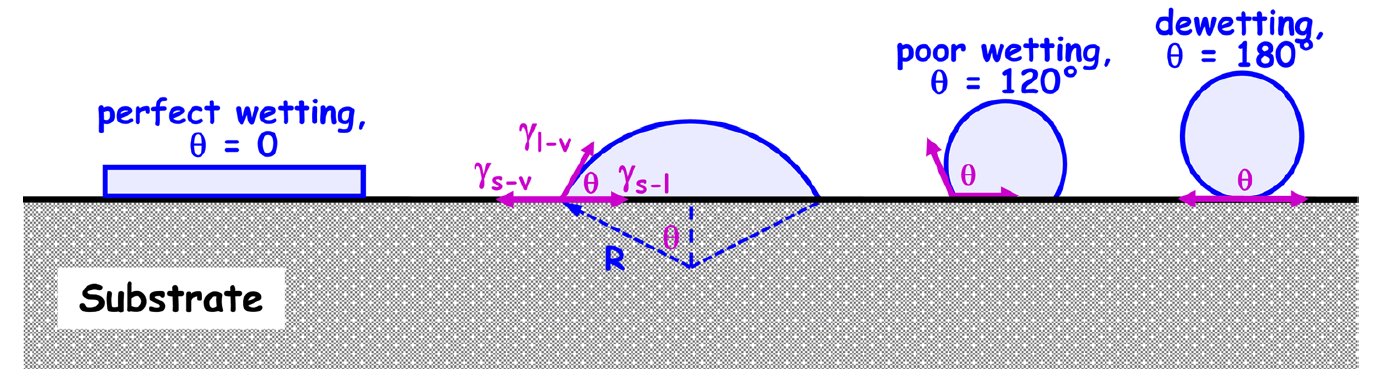
\includegraphics[width=\textwidth]{wetting.png}
		\captionof{figure}{Ilustrace povrchového napětí $\gamma$ a kontaktního 
		úhlu $\theta$.}
		\label{wetting}
	\end{center} 
\end{figure}
\par Povrchová energie materiálu je úměrná přilnavosti či fixaci na daný 
povrch. V praxi to znamená, že požadujeme vysokou povrchovou energii pro dobrou 
adhezi tiskařské barvy, lepidel, laků či nátěrů. Nízká povrchová energie je 
užitečná např. u skel na autě nebo u kuchyňského nádobí (pánví). Povrchová 
energie je vlastností materiálu, ale také jeho znečištěním, 
např. otisky prstů mohou snížit povrchovou energii.
\par Existuje několik metod, jak povrchovou energii určit. Nejjednodušší jsou 
fixy, které jsou kalibrované pro danou hodnotu povrchové energie. Pokud fix 
zanechá na povrchu malé kapičky, znamená to, že povrch má nižší povrchovou 
energii než je uvedená hodnota na fixu. Tato metoda se nejčastěji užívá v 
průmyslu, kde požadujeme, aby výrobek měl nižší (nebo vyšší) povrchovou energii 
než daná hodnota. Podobnou metodou jsou testovací inkousty. Jejich princip je 
stejný jako u fixů, kapalinu nanášíme štětečkem na povrch. Fixy ani inkousty 
nepotřebují přívod elektřiny či počítač, jsou ale drahé a mají krátkou 
životnost (3 až 6 měsíců).
\par Kapková metoda je založena na sledování tvaru kapky testovací kapaliny 
usazené na povrchu vzorku. Testovací kapaliny nesmí reagovat se vzorkem, musí 
mít známé a stálé parametry, neměly by být toxické, nesmí se rychle vypařovat a 
jejich povrchové napětí musí být vyšší než povrchová energie pevné látky. 
Výhodou této metody je určení hodnoty povrchové energie včetně chybové analýzy 
dle použitých modelů. Mezi chyby měření patří špatně usazená kapka, špatný fit 
profilu kapky, nehomogenita vzorku, sejmutí profilu před dosažením 
termodynamické rovnováhy, kontaminace měřicích kapalin aj.

\section{Praktická část}
\par Pro měření povrchové energie byl použit přístroj See System, viz 
obr.~\ref{ss}. Přístroj je složen ze stolku o~velikosti $10 \times 10$~cm, 
který lze dvěma stavěcími šrouby posouvat do všech směrů, a 2Mpix kamery, která 
snímá povrch. Na stolek se položí substrát, jehož povrchovou energii chceme 
zkoumat. Mikropipetou se nanese na povrch kapka a stolek se stavěcími šrouby 
naladí tak, aby kamera ostře snímala kapku na povrchu. Přístroj je připojen USB 
portem k~počítači, který pomocí příslušného softwaru dokáže ovládat kameru. 
Jakmile je kapka ostře vidět, přes software uložíme fotku z~kamery a dále 
zpracujeme. Na kapce zvolíme ručně tři body -- dvě na rozhraní pevná látka -- 
kapalina -- plyn a třetí bod na vrcholu kapky, čímž určíme kontaktní úhel pro 
danou testovací kapalinu, viz obr.~\ref{ssw}. Pokud toto uděláme pro kapky 
alespoň dvou různých kapalin, software dokáže spočítat povrchovou energii 
pomocí běžných modelů.

\par Měřili jsme povrchovou energii teflonu. Před měřením jsme povrch očistili 
isopropylalkoholem. Následně jsme měřili kontaktní úhel šesti testovacích 
kapalin: voda, etylenglykol, dijodometan, glycerol, formamid, 
$\alpha$-bromnaftalen, kde u každé kapaliny jsme naměřili kontaktní úhel 10 
kapek. Pro výpočet povrchové energie jsme použili několik 
metod.

\begin{figure}
	\begin{center}
		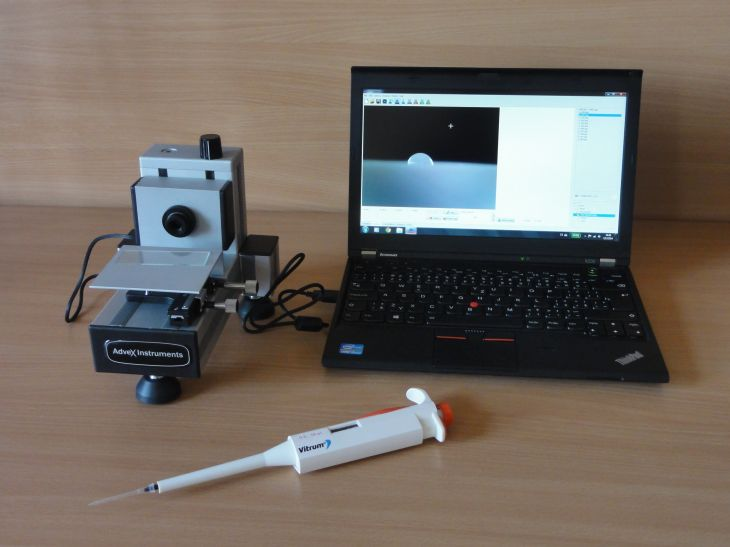
\includegraphics[width=\textwidth]{seesystem.jpg}
		\captionof{figure}{Přístroj See System pro měření kontaktního úhlu 
		kapky a určení povrchové energie.}
		\label{ss}
	\end{center} 
\end{figure}

\begin{figure}
	\begin{center}
		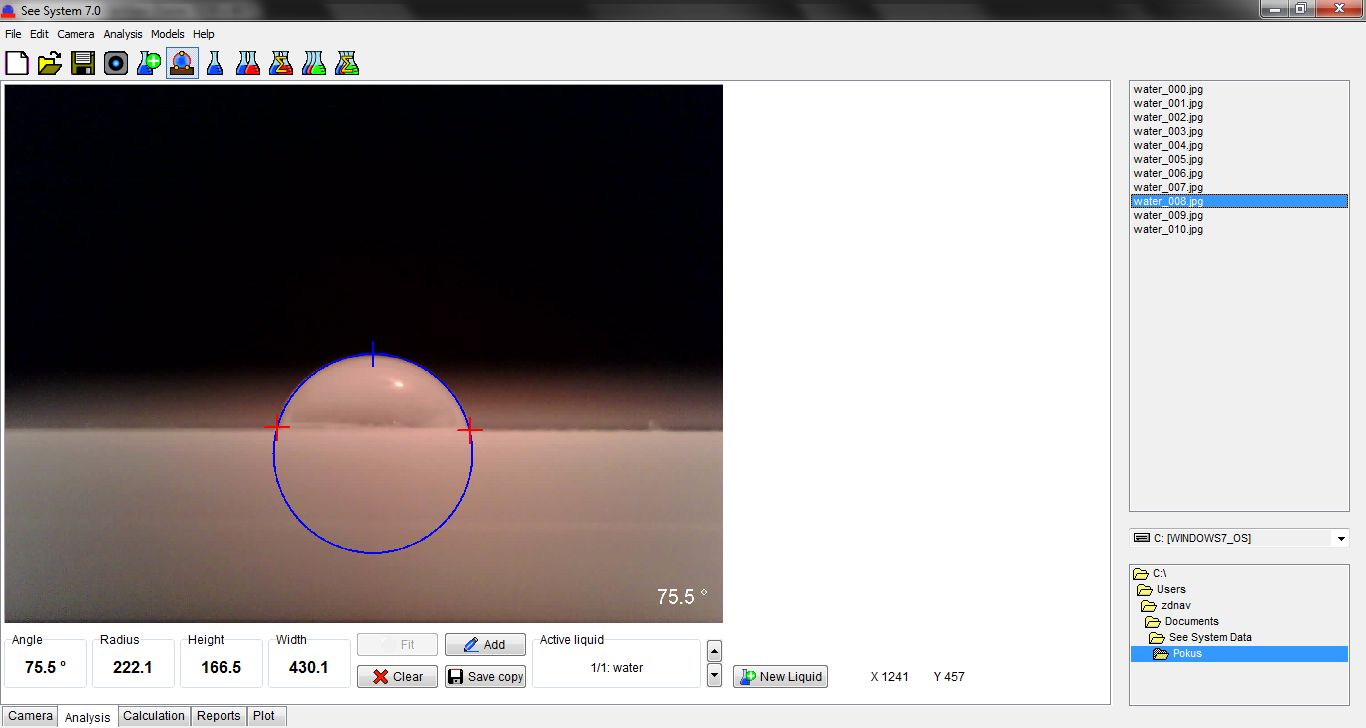
\includegraphics[width=\textwidth]{seesystemsw.jpg}
		\captionof{figure}{Ukázka tříbodového určení kontaktního úhlu pomocí 
		See System softwaru.}
		\label{ssw}
	\end{center} 
\end{figure}

%HODNOTY $\gamma_{\text{l}}$
%https://en.wikipedia.org/wiki/Surface-tension_values 
%https://en.wikipedia.org/wiki/Glycerol_(data_page)
%https://pubchem.ncbi.nlm.nih.gov/compound/formamide#section=Heat-of-Vaporization
%http://www.surface-tension.de/


\subsection{Zismanova metoda}
\par Zismanova metoda je založena na vynesení závislosti $\cos\theta = 
f\left(\gamma_{\text{l}} \right)$ do grafu. Po naměření kontaktních úhlů 
$\theta$ pro několik kapalin se známou hodnotou povrchové energie 
$\gamma_{\text{l}}$ (tab.~\ref{table1:surfTensionLiquid}) můžeme fitovat 
závislost rovnicí
\begin{equation}
	\cos\theta = 1 + 
	b \left( \gamma_{\text{c}} - \gamma_{\text{l}} \right)
\end{equation}
z které získáme hodnotu celkové povrchové energie $\gamma_{\text{c}}$.

\begin{table}[h]
	\caption{Povrchové napětí testovacích kapalin}
	\label{table1:surfTensionLiquid}
	\begin{tabular}{|c|c|}\hline
		kapalina  & $\gamma_{\text{l}}$\,[\si{\milli\newton\per\meter}]\\ \hline
		destilovaná voda   & 72,8                              \\
		etylenglykol       & 47,7                              \\
		dijodometan        & 50,8                              \\
		glycerol           & 64,0                              \\
		formamid           & 58,2                              \\
		$\alpha$-bromnaftalen & 44,4  \\ \hline
	\end{tabular}
\end{table}

\subsection{Wu metoda}
\begin{equation}
	\left(1+\cos\theta\right)\gamma_{\text{l}} = 
	4\left(\frac{\gamma_{\text{s}}^\text{d}\gamma_{\text{l}}^\text{d}}{\gamma_{\text{s}}^\text{d}
	 + \gamma_{\text{l}}^\text{d}} + 
	\frac{\gamma_{\text{s}}^\text{p}\gamma_{\text{l}}^\text{p}}{\gamma_{\text{s}}^\text{p}
	 + \gamma_{\text{l}}^\text{p}}\right)
\end{equation}
\par 

\subsection{Owens-Wendtova regresní metoda}
\begin{equation}
	\frac{1+\cos\theta}{2}\frac{\gamma_{\text{l}}}{\sqrt{\gamma_{\text{l}}^\text{d}}}
	 = \sqrt{\gamma_{\text{s}}^\text{d}} + \sqrt{\gamma_{\text{s}}^\text{p}} 
	 \sqrt{\frac{\gamma_{\text{l}}^\text{p}}{\gamma_{\text{l}}^\text{d}}}
\end{equation}
\par 

\subsection{Acidobazická metoda}
\begin{equation}
	\gamma = \gamma^{\text{LW}} + \gamma^{\text{AB}}
\end{equation}
\begin{equation}
	\gamma^{\text{AB}} = 2\sqrt{\gamma^+\gamma^-}
\end{equation}
\begin{equation}
		\left(1+\cos\theta\right)\gamma_{\text{l}} = 
		2\left(\sqrt{\gamma_\text{l}^{\text{LW}}\gamma_\text{s}^{\text{LW}}} + 
		\sqrt{\gamma_\text{l}^{\text{+}}\gamma_\text{s}^{\text{-}}} + 
		\sqrt{\gamma_\text{l}^{\text{-}}\gamma_\text{s}^{\text{+}}}\right)
\end{equation}
\par 

\subsection{Kwok-Neumann metoda}
\begin{equation}
	\cos\theta = -1 + 
2 {\left(\frac{\gamma_{\text{sv}}}{\gamma_{\text{lv}}}\right)}^{1/2} 
\left(1-0,0001057(\gamma_{\text{lv}} - \gamma_{\text{sv}})^2\right)
\end{equation}
\par 

\subsection{Li-Neumann metoda}
\begin{equation}
	\cos\theta = -1 + 
	2 {\left( \frac{\gamma_{\text{sv}}} {\gamma_{\text{lv}}} \right)}^{1/2} 
	\e^{-0,0001247(\gamma_{\text{lv}} - \gamma_{\text{sv}})^2}
\end{equation}
\par 





\section{Závěr}
V této úloze jsme se zabývali měřením povrchové energie. Konkrétně jsme měřili povrchovou energii teflonu pomocí přístroje See System. Pro výpočet povrchové energie jsme použili několik metod, vstupními parametry pro výslednou hodnotu byly námi naměřené kontaktní úhly šesti různých kapalin. První metodou byla Zismanova. Pro ni jsme k hodnotě získané ze softwaru See Systemu ... nafitovali danou závislost i ručně, přičemž nám vyšlo ... . Obě hodnoty se v rámci chyby shodují, ta je ovšem příliš velká a tato metoda se tedy jeví jako nevhodná.

\end{document}
